\documentclass{article}
\usepackage[letterpaper, margin=1in]{geometry}
\usepackage{ragged2e}
\usepackage[hidelinks]{hyperref}
\usepackage{booktabs}
\usepackage{tabularx}
\usepackage{titling}
\usepackage{setspace}
\usepackage{tikz}
\usepackage{graphicx} % Include graphic importing
\graphicspath{{images/}}
\newcommand{\subtitle}[1]{%
  \posttitle{%
    \par\end{center}
    \begin{center}\large#1\end{center}
    \vskip0.5em}%
}
\usepackage{listings}
\usepackage{color}
\definecolor{dkgreen}{rgb}{0,0.6,0}
\definecolor{gray}{rgb}{0.5,0.5,0.5}
\definecolor{mauve}{rgb}{0.58,0,0.82}
\lstset{frame=tb,
  language=Java,
  aboveskip=3mm,
  belowskip=3mm,
  showstringspaces=false,
  columns=flexible,
  basicstyle={\small\ttfamily},
  numbers=none,
  numberstyle=\tiny\color{gray},
  keywordstyle=\color{blue},
  commentstyle=\color{dkgreen},
  stringstyle=\color{mauve},
  breaklines=true,
  breakatwhitespace=true,
  tabsize=3
}
\usepackage{float}
\usepackage{cite}
\usepackage[toc,nonumberlist,acronym]{glossaries}
\newglossary[blg]{beer}{bls}{blo}{Beer Terminology}
\newglossary[tlg]{technical}{tls}{tlo}{Technical Terminology}
\makeglossaries

\newglossaryentry{grist}{type=beer, name=Grist, text=grist, description=The combination of milled grains to be used in a particular brew. Also sometimes applied to hops \cite{beer-terms}.}
\newglossaryentry{mash}{type=beer, name=Mash, text=mash, description=(Verb) To release malt sugars by soaking the grains in water. (Noun) The resultant mixture \cite{beer-terms}.}
\newglossaryentry{pitch}{type=beer, name=Pitch, text=pitch, description=To add yeast.}
\newglossaryentry{sparge}{type=beer, name=Sparge, text=sparge, description=To spray grist with hot water in order to remove soluble sugars (maltose). This takes place at the end of the mash \cite{beer-terms}.}
\newglossaryentry{trub}{type=beer, name=Trub, text=trub, description=The layer of sediment that appears at the bottom of the fermentation vessel upon the completion of fermentation.}
\newglossaryentry{wort}{type=beer,name=Wort, text=wort, description=The solution of grain sugars strained from the mash tun \cite{beer-terms}.}

\newglossaryentry{rpi}{type=technical, name=Raspberry Pi 2 Model B, text=Raspberry Pi, description=The Raspberry Pi 2 Model B is the second generation Raspberry Pi. It replaced the original Raspberry Pi 1 Model B+ in February 2015.}

%\newacronym{abv}{ABV}{Alcohol By Volume}
\newacronym{arm}{ARM}{Acorn \gls{risc} Machine}
\newacronym{i2c}{I2C}{Inter-Integrated Circuit}
\newacronym{json}{JSON}{JavaScript Object Notation}
\newacronym{lamp}{LAMP}{Lamp Apache MySQL PHP}
\newacronym{lts}{LTS}{Long Term Support}
\newacronym{ram}{RAM}{Random Access Memory}
\newacronym{risc}{RISC}{Reduced Instruction Set Computing}
\newacronym{ros}{ROS}{Robot Operating System}

\author{\\\\}
\title{Brew It Yourself}
\subtitle{An Automated Single-Vessel Home Brewery System}

\begin{document}

\begin{titlepage}
    \begin{center}
        \vspace*{1cm}
        
        \textsc{\LARGE University of Waterloo}\\ [0.1cm]
        \textsc{\Large Faculty of Engineering}\\
        \textsc{Department of Electrical and Computer Engineering}

		\vspace{4.5cm}

        \textsc{\Huge \textbf{Brew It Yourself}}
        
        \vspace{0.2cm}
        An Automated Single Vessel Home Brewery System
                
        \vfill
        
        Group Number: 2016.019
		\\Consultant: Douglas Harder
        \vspace{0.5cm}
        \\Kevin Nause (20413332) 
        \\Mathieu Tremblay (20420813) 
        \\Scott Wood (20379649) 
        \\Steve Jung (20411563) 
        \vspace{0.5cm}
        \\Date: \today
        \vspace{3.0cm}
    \end{center}
\end{titlepage}

\pagebreak
\tableofcontents
%\listoffigures
%\listoftables
\pagebreak
\justify
\onehalfspacing
\section{High-Level Description of Project}
\subsection{Motivation}
The art of home brewing has been steadily gaining popularity over the past 35 years alongside the rise of craft breweries in North America, so much so that in 2010 there were over 2000 craft breweries in the United States, after starting with only 8 in 1980 \cite{craft-beer}. The traditional method for homebrewing requires various components, constant monitoring and heavy maintenance. There should be a solution which reduces complexity, making it much more affordable and practical for home use. We hope to create a single vessel system that would make the home brewing process precise, automated and compact, all at a reasonable price.
\subsection{Project Objective}
The objective of this project is to combine homebrewing experience with engineering design, and construct a single vessel brewing system. By maintaining a strict control of key parameters, the brewing process is regulated using a combination of fluid mechanics, heat transfer, digital controls, power systems, embedded robotics and mobile development. The Robotics Operating System (ROS), allows for a design where sensors can be added to a modular setup and provide feedback. By receiving feedback from temperature readings, density measurements and pH monitoring, the brewing process can be accurately recorded, shared, and automated by the system. 
\subsection{Block Diagram}
Figure \ref{fig:block} shows relevant links between the physical, mechanical design of the brewing system, as well as the computer systems and their underlying software.

\begin{figure}[H]
\begin{center}
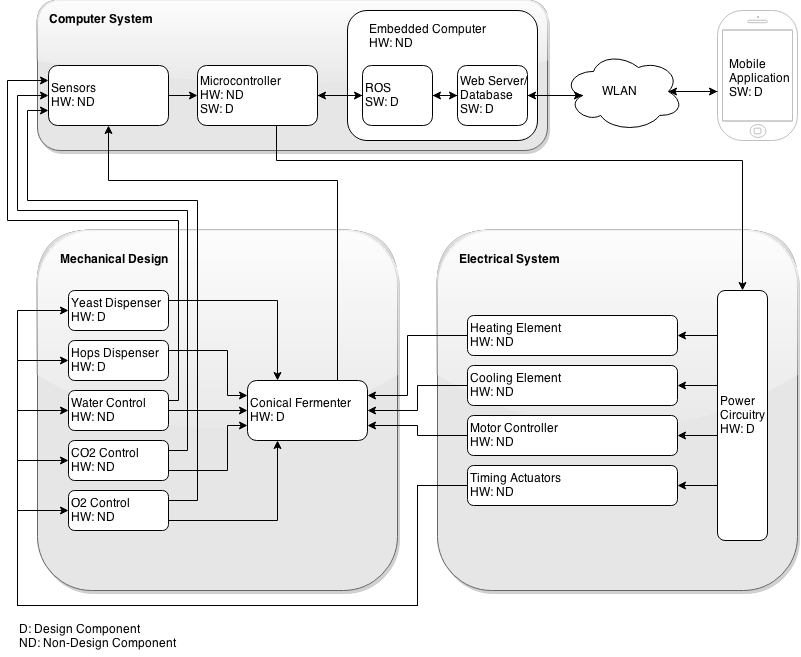
\includegraphics[scale=0.58]{block-diagram.png}
\caption{Block Diagram outlining the interactions between the computer, electrical, and mechanical systems}
\label{fig:block}
\end{center}
\end{figure}

\subsubsection{Description of System}
The single vessel brewing system, as shown in Figure \ref{fig:block}, contains various sensors which forward the environmental parameters to the microcontroller. The data from the various sensors accurately represents the state of the fermenter and feed into digital control loops running on the microcontroller.  Data from sensor modules is obtained by a microcontroller via an I2C interface. This data is then sent to an embedded computer system over USB where it is logged in a database and used to control relevant subsystems. Control commands are sent from the embedded computer to the microcontroller, where the appropriate component can be communicated with in order to regulate the brewing environment.  The embedded computer system is then able to send diagnostic information and push notifications to a mobile device through a WLAN connection.

\subsubsection{Designing and Not Designing Components}
The following is an outline of the components in the block diagram and the requirements associated for each Designing (D) and Non-Designing (ND) component.

\begin{itemize}
\item\textbf{Sensors}
\\ND: Sensors being used in the vessel are not being designed.  Instead, off-the-shelf sensors are being purchased and integrated into the system.  Relevant sensor types for this system include, but aren’t limited to, pH sensors, volume sensors, flow meters, temperature probes, etc.

\item\textbf{Microcontroller(s)}
ND: The hardware of the microcontroller is not being designed since that’s outside the scope of this project. The system instead uses an off-the-shelf microcontroller.
D: The software running on the microcontroller is being designed. This software mainly consists of digital control loops for interfacing with the sensors and power electronic circuitry.

\item\textbf{Conical Fermentation Vessel}
\\D: The mechanical features and dimensions of the conical fermentation vessel are being designed to hold various sensors and other electrical and mechanical components. 

\item\textbf{Power Electronic Circuitry}
\\D: The power electronic circuitry is being designed to power the pumps, motors, actuators, and heating/cooling mechanisms. The circuitry takes input from the digital controller running on the microcontroller and outputs the appropriate power to the end devices.

\item\textbf{Heating and Cooling Elements}
\\ND: The heating coils and refrigeration unit used to regulate temperature of the vessel are not being designed. Instead, off-the-shelf or salvaged and adapted components from existing appliances (e.g. hot water tank coils, home air conditioning heat pump) are being used and the power electronic circuitry is being designed to power these devices.

\item\textbf{Motor Controller}
\\ND: The motors, pumps, and mixing mechanisms used in our system are not being designed. Instead, off-the-shelf or salvaged and adapted components from existing appliances (e.g. blender mixing prop, aquarium pumps) are being used and the power electronic circuitry is being designed to power these devices.

\item\textbf{Timing actuators}
\\ND: The actuators used in our system are not being designed. Instead, off-the-shelf solenoids and servo motors are being used and the mechanical subsystems that they will actuate are being designed. The power electronic circuitry is also being deigned to be able to power the actuators.

\item\textbf{Embedded Computer System}
\\ND: The hardware and operating system of the embedded computer system is not a design objective as it is outside the scope of this project. Instead an off-the-shelf embedded computer is purchased and a Debian based Linux operating system is installed to satisfy the requirements for the development environment.
\\D: The embedded computer system is configured with a Web Server, Database, and the Robotics Operating System (ROS).  Microcontrollers can be modularly added to the system via USB and automatically configured as ROS nodes through negotiations.

\item\textbf{Mobile Application}
\\D: The mobile application is designed such that the user can receive push notifications and see various sensor data during the brew process.
\end{itemize}

\section{Project Specifications}
This section outlines the functional and non-functional requirements of the project design.
\subsection{Functional Specifications}
Table \ref{tab:func} describes each functional requirement and highlights whether it is essential or not to the completion of the project.

\newcolumntype{Z}{>{\raggedright\arraybackslash}X}
\begin{table}[H]
\centering
\begin{tabularx}{\textwidth}{l l Z}
\toprule
\textbf{Specification} & \textbf{Classification} & \textbf{Description} \\ 
\midrule
Completion of the Brewing Process
& Essential	
& The device automatically completes the brewing process, consisting of these steps:
\begin{itemize}
\item \Gls{mash}
\item \Gls{sparge}
\item Boil \Gls{wort}
\item Dispense Hops
\item Aerate the \Gls{wort}
\item \Gls{pitch} the Yeast
\item Kegging and Dispensing
\end{itemize}
\noindent in its entirety and in the correct order.  For more information on the brewing process and the terms used, please see the Glossary.
\\\\
Heating Unit
& Essential
& Mashing the grains, sparging the \gls{grist}, and boiling the \gls{wort} all require high water temperatures. The system is able to accurately heat the contents to a minimum of 110$^{\circ}$C within 1$^{\circ}$C of error.
\\
\end{tabularx}
\end{table}

\begin{table}[H]
\centering
\begin{tabularx}{\textwidth}{l l Z}
Cooling Unit
& Essential
& Yeast pitching and fermentation happen immediately after boiling the wort, but require temperatures a specific temperature (typically 20$^{\circ}$C). The system is able to rapidly cool the wort to a temperature within 1$^{\circ}$C of the target temperature so that the yeast may be pitched safely.
\\\\
Temperature Regulation
& Essential
& The system is able to control temperature for each step in the brewing process.  An error of 1$^{\circ}$C is the target specification.
\\\\
\Gls{trub} Removal
& Non-Essential
& Remove the undesired sediment and other byproducts at the bottom of the fermenter so that ageing may take place within the vessel.  The user does not have to maintain the \gls{trub} accumulated by the brewing process.
\\\\
Application Notifications
& Non-Essential
& The system provides notifications to the user updating them on the current state or action being taken.  Additionally errors or warnings can be sent, in cases of emergency such as clogs, low oxygen or carbon dioxide, or an improper environment.
\\\\
Database
& Essential
& The system is able query the specific steps it needs to automate for a specific brew.  Additionally, it can store various data involved in brewing including temperature, pH levels and density measurements to generate logs and reports.
\\\\
Reproducibility
& Non-Essential
& The system is able to record recipes, ingredients and steps for various brews. The user can recreate the same type of brew if they select one of the recipes.
\\
\bottomrule
\end{tabularx}
\caption{An overview of each functional specification of the project}
\label{tab:func}
\end{table}

\pagebreak
\subsection{Non-Functional Specifications}
Table \ref{tab:non-func} describes each non-functional requirement and highlights whether it is essential or not to the completion of the project.

\begin{table}[H]
\centering
\begin{tabularx}{\textwidth}{l l Z}
\toprule
\textbf{Specification} & \textbf{Classification} & \textbf{Description} \\ 
\midrule
Temperature Accuracy
& Essential
& The system accurately regulates the temperature required for the brewing process within 1$^{\circ}$C of the targeted temperature.
\\\\
Volume Control
& Essential
& The end result must be greater than or equal to the target yield volume.  Target yields typically consist of 15.5 gallons, 7.75 gallons, and 5.16 gallons.  These are the standard sizes of a half barrel keg, quarter barrel keg, and a sixth barrel keg respectively.
\\\\
Size
& Essential
& The dimensions are limited such that the vessel can fit within a standard 36 inch residential door frame.
\\\\
Mobility
& Essential
& The system is able to be relocated by a single person using the aid of caster wheels and or a standard 18 inch wide utility dolly.
\\\\
Sanitation
& Essential
& The system employs SUS 304 stainless steel to maintain food-grade sanitation conditions.  The vessel is self cleaning since a sanitary environment is crucial for the brewing process.
\\
\bottomrule
\end{tabularx}
\caption{An overview of each non-functional specification of the project}
\label{tab:non-func}
\end{table}
\pagebreak
\section{Risk Assessment}
Table \ref{tab:risk} describes each risk associated with the project and highlights methods and actions to take to mitigate any adverse effects.

\begin{table}[H]
\centering
\begin{tabularx}{\textwidth}{Z l l Z}
\toprule
\textbf{Risk} & \textbf{Impact} & \textbf{Probability} &\textbf{Mitigation} \\ 
\midrule
Funding this project proves costly and infeasible due to the requirement of expensive components
& High
& High
& Sources of additional funding and sponsorship are being investigated at an early stage of this project to mitigate this risk.
\\\\
The on-campus machine shops have insufficient manufacturing capability and precision to create the conical vessel
& High
& Medium
& Communications with the on-campus machine shop is happening at an early stage of the project, so that if necessary there is time to investigate alternative manufacturers.
\\\\
Latencies in the supply chain caused by shipping overseas cause crucial parts to arrive too close to the prototype deadline
& High
& Low
& Local suppliers for necessary parts and components are being considered first before any overseas suppliers.
\\\\
Poor quality or malfunctioning sensors cause unreliable control of the brewing process
& Medium
& High
& The use of higher quality sensors or multiple redundant sensors can lower this risk.
\\
\bottomrule
\end{tabularx}
\caption{An overview of each risk associated with the project}
\label{tab:risk}
\end{table}

\section{Detailed Design}
\subsection{Mechanical Design}
\subsubsection{Material}
\subsubsection{Tank Structure}

\subsection{Electrical System}
\subsubsection{Heating and Cooling Controller}
\subsubsection{Motor Controller}
\subsubsection{Timing Actuators}

\subsection{Computer System}
The computer systems consist of three main components, the embedded central computer, the micro-controller and sensor pairs, as well as a Web Server and Database pair to allow for storage and communications.  The detailed description of each subcomponent and the methods of interaction between them is discussed in this section.
\subsubsection{Embedded Computer}
The primary function of the embedded computer system is to aggregate data in close to real-time from the multiple sensors used in the design.  Analysis of this data is crucial for determining the current progress in the \gls{mash}, \gls{sparge}, and boiling of the \gls{wort}.  For specific analysis of sensor data please see subsection \ref{subsec:sensor}.

For ease of repeatability, availability, and cost the \gls{rpi} was selected.  At the time of design and creation of this report, this is the most recent hardware revision of the \gls{rpi}.  The relevant hardware specifications for the \gls{rpi} is a quad-core \gls{arm} processor, 1GB of \gls{ram}, and a Bluetooth dongle for local wireless communications (rated to 50m).  Since the outer shell of the fermenter is aluminum, the casing for the \gls{rpi} can act as a heat sink, allowing it to be safely overclocked to 1GHz, 500MHz, and 500MHz for the \gls{arm} processor frequency, sdram frequency, and L2 cache (core) frequency respectively.  The configuration file below allows for a substantial performance boost with negligible thermal impact.  

\begin{lstlisting}
arm_freq=1000
sdram_freq=500
core_freq=500
over_voltage=2
arm_freq_min=400
sdram_freq_min=250
core_freq_min=250
\end{lstlisting}

For a list of stock specifications and configurations for the \gls{rpi}, please see Appendix \ref{app:rpi}.  The operating system chosen was the \gls{arm} build of Ubuntu 14.04 \gls{lts}, codename Trusty Tahr, as well as \gls{ros} Jade Turtle for sensor coordination and communication.  Ubuntu 14.04 was chosen over the default Raspbian operating system for increased security due to the use of SELinux policies.  Since the \gls{rpi} will be acting as a LAMP server as well for mobile interaction and remote notifications, enforcing read only access over the configured port of choice is a necessity. For an in depth overview of the mobile application please see subsection \ref{subsec:mobile-app}.  Additionally, the \gls{lts} version of Ubuntu was chosen for a maximum of five years support, as well as increased compatibility and reliability for repository packages specific to the trusty distribution.

\subsubsection{Sensors and Micro-Controllers}\label{subsec:sensor}
Every sensor in the system is paired with a micro-controller to enable a modular design and a plug and play like support.  By adding more sensors to the system, more information can be provided as feedback to enable better logging and regulation of the brewing environment.  The only mandatory sensors for the system are a main temperature sensor for the \gls{wort} and flow meters on the liquid inputs and outputs of the system.  By introducing additional sensors, such as pH and density sensors, certain yield thresholds of interest in the \gls{sparge} and fermentation procedure can be met rather than approximated.  Additionally, this will allow for a tier based configuration for the automated vessel to reduce cost and complexity if desired.  As the end goal for this project is to have a community influenced input, having a customizable sensor configuration with open hardware and software pairs is encouraged.  For maximum affordability the Arduino compatible Teensy-LC microcontroller is used to poll the sensors and report data, however any Arduino compatible microcontroller may be used.  Technical specifications for the Teensy-LC microcontroller can be seen in Appendix \ref{app:teensy}  The bridge between the \gls{ros} instance on the \gls{rpi} and the Arduino compatible microcontroller is achieved through the use of the ROSserial package.  Example code for obtaining data from a TMP102 temperature sensor over \gls{i2c} at address 0x91 \cite{tmp102} can be seen below \cite{rosserial}.

\begin{lstlisting}
#include <Wire.h>
#include <ros.h>
#include <std_msgs/Float32.h>

//Set up the ros node and publisher
std_msgs::Float32 temp_msg;
ros::Publisher pub_temp("temperature", &temp_msg);
ros::NodeHandle nh;

int sensorAddress = 0x91 >> 1;  // From datasheet
long publisher_timer;

void setup()
{
  Wire.begin();        // join i2c bus (address optional for master)
  nh.initNode();
  nh.advertise(pub_temp);
}

void loop()
{
  if (millis() > publisher_timer) {
  // step 1: request reading from sensor
    Wire.requestFrom(sensorAddress,2);
    delay(10);
    if (2 <= Wire.available())  // if two bytes were received
    {
      byte msb;
      byte lsb;
      int temperature;

      msb = Wire.read();  // receive high byte (full degrees)
      lsb = Wire.read();  // receive low byte (fraction degrees)
      temperature = ((msb) << 4);  // MSB
      temperature |= (lsb >> 4);   // LSB

      temp_msg.data = temperature*0.0625;
      pub_temp.publish(&temp_msg);
    }
  publisher_timer = millis() + 1000; //publish once a second
  }
  nh.spinOnce();
}
\end{lstlisting}

Additionally, controllers can be linked to the system via Arduino compatible micro-controllers and receive inputs based on sensor data gathered via \gls{ros} publications.  To improve the resolution or accuracy of data and controls, the polling interval of each of the micro-controllers can be calibrated appropriately.  Since most sensors will remain idle for a majority of the brewing process, their sampling rates can be scaled using a simple algorithm as suggested in the code sample below.

\begin{lstlisting}
#include <std_msgs/Float32.h>

int sample_rate = MIN_SAMPLE_RATE;
int sample_count = 0;

void scale_rate(std_msgs::Float32 prev, std_msgs::Float32 curr)
{
    if(prev == curr)
    {
        sample_count++;
    }
    else
	{
        sample_count--;
	}

	if(sample_count == SCALE_THRESHOLD)
	{
   		sample_rate = increase_rate();
    	sample_count = SCALE_THRESHOLD >> 1;
	}
	else if(sample_count == 0)
	{
    	sample_rate = decrease_rate();
    	sample_count = SCALE_THRESHOLD >> 1;
	}
}
\end{lstlisting}

The two fundamental controllers that require communications for the operation of the system are the water controller and the heating and cooling controllers.  Figure \ref{fig:water-controller} demonstrates a state diagram for the water controller and Figure \ref{fig:temperature-controller} demonstrate the state diagrams for toggling the heating and cooling states of the temperature controller.  The variables volume, temp, target and offset represent the current volume, current temperature, desired resultant, and amount of allowed deviation from target respectively.

\begin{figure}[H]
\begin{center}
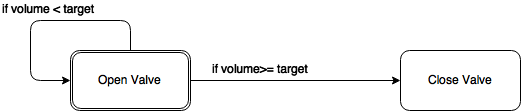
\includegraphics[scale=0.50]{water-controller-state-diagram.png}
\caption{State diagram for the water controller component}
\label{fig:water-controller}
\end{center}
\end{figure}

\begin{figure}[H]
\begin{center}
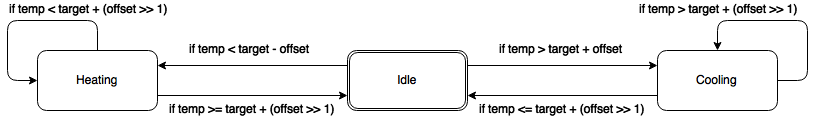
\includegraphics[scale=0.50]{temperature-controller-state-diagram.png}
\caption{State diagram for the temperature controller component}
\label{fig:temperature-controller}
\end{center}
\end{figure}

\subsubsection{Web Server and Database}
A \gls{lamp} server is the current solution for delivering information from the embedded computer to the mobile application.  All communications and parameters are to be communicated using a \gls{json} format.  The database will consist of relational connections between recipes, instructions, ingredients, sensors, and logged data as demonstrated in Figure \ref{fig:database-diagram}.

\begin{figure}[H]
\begin{center}
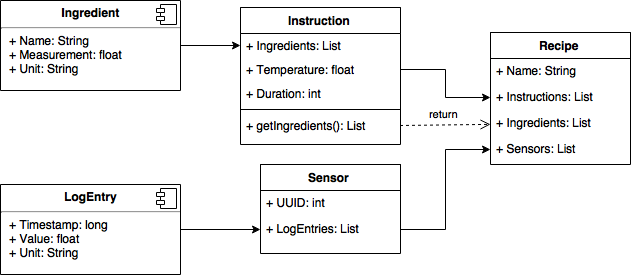
\includegraphics[scale=0.50]{database-uml-diagram.png}
\caption{A UML diagram showing the relation between tables and their entries in the logging database}
\label{fig:database-diagram}
\end{center}
\end{figure}

\subsection{Mobile Application}
\subsubsection{Real Time Data Analysis}
\subsubsection{Input Controls and Interaction}

\section{Discussion and Project Timeline}
\subsection{Evaluation of Final Design}
\subsection{Use of Advanced Knowledge}
\subsection{Creativity, Novelty, Elegance}
\subsection{Student Hours}
\subsection{Potential Safety Hazards}
\subsection{Project Timeline}

\pagebreak
\printglossary[type=acronym]
\printglossary[type=beer]
\printglossary[type=technical]

\bibliography{specifications-bib}{}
\bibliographystyle{ieeetr}

\end{document}